\documentclass[twoside]{book}

% Packages required by doxygen
\usepackage{fixltx2e}
\usepackage{calc}
\usepackage{doxygen}
\usepackage[export]{adjustbox} % also loads graphicx
\usepackage{graphicx}
\usepackage[utf8]{inputenc}
\usepackage{makeidx}
\usepackage{multicol}
\usepackage{multirow}
\PassOptionsToPackage{warn}{textcomp}
\usepackage{textcomp}
\usepackage[nointegrals]{wasysym}
\usepackage[table]{xcolor}

% Font selection
\usepackage[T1]{fontenc}
\usepackage[scaled=.90]{helvet}
\usepackage{courier}
\usepackage{amssymb}
\usepackage{sectsty}
\renewcommand{\familydefault}{\sfdefault}
\allsectionsfont{%
  \fontseries{bc}\selectfont%
  \color{darkgray}%
}
\renewcommand{\DoxyLabelFont}{%
  \fontseries{bc}\selectfont%
  \color{darkgray}%
}
\newcommand{\+}{\discretionary{\mbox{\scriptsize$\hookleftarrow$}}{}{}}

% Page & text layout
\usepackage{geometry}
\geometry{%
  a4paper,%
  top=2.5cm,%
  bottom=2.5cm,%
  left=2.5cm,%
  right=2.5cm%
}
\tolerance=750
\hfuzz=15pt
\hbadness=750
\setlength{\emergencystretch}{15pt}
\setlength{\parindent}{0cm}
\setlength{\parskip}{3ex plus 2ex minus 2ex}
\makeatletter
\renewcommand{\paragraph}{%
  \@startsection{paragraph}{4}{0ex}{-1.0ex}{1.0ex}{%
    \normalfont\normalsize\bfseries\SS@parafont%
  }%
}
\renewcommand{\subparagraph}{%
  \@startsection{subparagraph}{5}{0ex}{-1.0ex}{1.0ex}{%
    \normalfont\normalsize\bfseries\SS@subparafont%
  }%
}
\makeatother

% Headers & footers
\usepackage{fancyhdr}
\pagestyle{fancyplain}
\fancyhead[LE]{\fancyplain{}{\bfseries\thepage}}
\fancyhead[CE]{\fancyplain{}{}}
\fancyhead[RE]{\fancyplain{}{\bfseries\leftmark}}
\fancyhead[LO]{\fancyplain{}{\bfseries\rightmark}}
\fancyhead[CO]{\fancyplain{}{}}
\fancyhead[RO]{\fancyplain{}{\bfseries\thepage}}
\fancyfoot[LE]{\fancyplain{}{}}
\fancyfoot[CE]{\fancyplain{}{}}
\fancyfoot[RE]{\fancyplain{}{\bfseries\scriptsize Generated by Doxygen }}
\fancyfoot[LO]{\fancyplain{}{\bfseries\scriptsize Generated by Doxygen }}
\fancyfoot[CO]{\fancyplain{}{}}
\fancyfoot[RO]{\fancyplain{}{}}
\renewcommand{\footrulewidth}{0.4pt}
\renewcommand{\chaptermark}[1]{%
  \markboth{#1}{}%
}
\renewcommand{\sectionmark}[1]{%
  \markright{\thesection\ #1}%
}

% Indices & bibliography
\usepackage{natbib}
\usepackage[titles]{tocloft}
\setcounter{tocdepth}{3}
\setcounter{secnumdepth}{5}
\makeindex

% Hyperlinks (required, but should be loaded last)
\usepackage{ifpdf}
\ifpdf
  \usepackage[pdftex,pagebackref=true]{hyperref}
\else
  \usepackage[ps2pdf,pagebackref=true]{hyperref}
\fi
\hypersetup{%
  colorlinks=true,%
  linkcolor=blue,%
  citecolor=blue,%
  unicode%
}

% Custom commands
\newcommand{\clearemptydoublepage}{%
  \newpage{\pagestyle{empty}\cleardoublepage}%
}

\usepackage{caption}
\captionsetup{labelsep=space,justification=centering,font={bf},singlelinecheck=off,skip=4pt,position=top}

%===== C O N T E N T S =====

\begin{document}

% Titlepage & ToC
\hypersetup{pageanchor=false,
             bookmarksnumbered=true,
             pdfencoding=unicode
            }
\pagenumbering{alph}
\begin{titlepage}
\vspace*{7cm}
\begin{center}%
{\Large Factory\+Method }\\
\vspace*{1cm}
{\large Generated by Doxygen 1.8.13}\\
\end{center}
\end{titlepage}
\clearemptydoublepage
\pagenumbering{roman}
\tableofcontents
\clearemptydoublepage
\pagenumbering{arabic}
\hypersetup{pageanchor=true}

%--- Begin generated contents ---
\chapter{Namespace Index}
\section{Packages}
Here are the packages with brief descriptions (if available)\+:\begin{DoxyCompactList}
\item\contentsline{section}{\hyperlink{namespace_decorator}{Decorator} }{\pageref{namespace_decorator}}{}
\end{DoxyCompactList}

\chapter{Hierarchical Index}
\section{Class Hierarchy}
This inheritance list is sorted roughly, but not completely, alphabetically\+:\begin{DoxyCompactList}
\item \contentsline{section}{Strategy.\+Dojazd}{\pageref{interface_strategy_1_1_dojazd}}{}
\begin{DoxyCompactList}
\item \contentsline{section}{Strategy.\+Rower}{\pageref{class_strategy_1_1_rower}}{}
\item \contentsline{section}{Strategy.\+Samochod}{\pageref{class_strategy_1_1_samochod}}{}
\end{DoxyCompactList}
\item \contentsline{section}{Strategy.\+Praca}{\pageref{interface_strategy_1_1_praca}}{}
\begin{DoxyCompactList}
\item \contentsline{section}{Strategy.\+Maluje\+Samochod}{\pageref{class_strategy_1_1_maluje_samochod}}{}
\item \contentsline{section}{Strategy.\+Montuje\+Silnik}{\pageref{class_strategy_1_1_montuje_silnik}}{}
\item \contentsline{section}{Strategy.\+Testuje\+Samochodow}{\pageref{class_strategy_1_1_testuje_samochodow}}{}
\end{DoxyCompactList}
\item \contentsline{section}{Strategy.\+Pracownik}{\pageref{class_strategy_1_1_pracownik}}{}
\item \contentsline{section}{Strategy.\+Spedzanie\+Wolnego\+Czasu}{\pageref{interface_strategy_1_1_spedzanie_wolnego_czasu}}{}
\begin{DoxyCompactList}
\item \contentsline{section}{Strategy.\+Gra\+Komputerowa}{\pageref{class_strategy_1_1_gra_komputerowa}}{}
\item \contentsline{section}{Strategy.\+Literatura\+Popularno\+Naukowa}{\pageref{class_strategy_1_1_literatura_popularno_naukowa}}{}
\item \contentsline{section}{Strategy.\+Silownia}{\pageref{class_strategy_1_1_silownia}}{}
\end{DoxyCompactList}
\item \contentsline{section}{Strategy.\+Strategy}{\pageref{class_strategy_1_1_strategy}}{}
\end{DoxyCompactList}

\chapter{Class Index}
\section{Class List}
Here are the classes, structs, unions and interfaces with brief descriptions\+:\begin{DoxyCompactList}
\item\contentsline{section}{\hyperlink{class_lazy_1_1_custom_lazy_class}{Lazy.\+Custom\+Lazy\+Class} \\*\hyperlink{class_lazy_1_1_custom_lazy_class}{Custom\+Lazy\+Class} posiada zmienna \+\_\+\+Value inicjalizowaną tuż przed uzyciem }{\pageref{class_lazy_1_1_custom_lazy_class}}{}
\item\contentsline{section}{\hyperlink{class_lazy_1_1_lazy}{Lazy.\+Lazy} \\*Klasa zawierająca funkcje Main }{\pageref{class_lazy_1_1_lazy}}{}
\item\contentsline{section}{\hyperlink{class_lazy_1_1_lazy_class}{Lazy.\+Lazy\+Class} \\*\hyperlink{class_lazy_1_1_lazy_class}{Lazy\+Class} posiada zmienna Value }{\pageref{class_lazy_1_1_lazy_class}}{}
\end{DoxyCompactList}

\chapter{Namespace Documentation}
\hypertarget{namespace_factory_method}{}\section{Factory\+Method Namespace Reference}
\label{namespace_factory_method}\index{Factory\+Method@{Factory\+Method}}
\subsection*{Classes}
\begin{DoxyCompactItemize}
\item 
class \hyperlink{class_factory_method_1_1_factory_method}{Factory\+Method}
\begin{DoxyCompactList}\small\item\em Klasa zawierająca funkcje Main \end{DoxyCompactList}\item 
class \hyperlink{class_factory_method_1_1_osobowy}{Osobowy}
\begin{DoxyCompactList}\small\item\em Produkt sprecyzowany 1 \end{DoxyCompactList}\item 
class \hyperlink{class_factory_method_1_1_producent_samochodow}{Producent\+Samochodow}
\begin{DoxyCompactList}\small\item\em Producent tworzący obiekty na podstawie parametru about \end{DoxyCompactList}\item 
class \hyperlink{class_factory_method_1_1_samochod}{Samochod}
\begin{DoxyCompactList}\small\item\em Ogolny produkt \end{DoxyCompactList}\item 
class \hyperlink{class_factory_method_1_1_sportowy}{Sportowy}
\begin{DoxyCompactList}\small\item\em Produkt sprecyzowany 3 \end{DoxyCompactList}\item 
class \hyperlink{class_factory_method_1_1_terenowy}{Terenowy}
\begin{DoxyCompactList}\small\item\em Produkt sprecyzowany 2 \end{DoxyCompactList}\end{DoxyCompactItemize}

\chapter{Class Documentation}
\hypertarget{class_factory_method_1_1_factory_method}{}\section{Factory\+Method.\+Factory\+Method Class Reference}
\label{class_factory_method_1_1_factory_method}\index{Factory\+Method.\+Factory\+Method@{Factory\+Method.\+Factory\+Method}}


Klasa zawierająca funkcje Main  


\subsection*{Static Public Member Functions}
\begin{DoxyCompactItemize}
\item 
\mbox{\Hypertarget{class_factory_method_1_1_factory_method_a56c9c647f5dad0aeb51e21927aa4af85}\label{class_factory_method_1_1_factory_method_a56c9c647f5dad0aeb51e21927aa4af85}} 
static void {\bfseries Main} (string\mbox{[}$\,$\mbox{]} args)
\end{DoxyCompactItemize}


\subsection{Detailed Description}
Klasa zawierająca funkcje Main 



The documentation for this class was generated from the following file\+:\begin{DoxyCompactItemize}
\item 
Program.\+cs\end{DoxyCompactItemize}

\hypertarget{class_factory_method_1_1_osobowy}{}\section{Factory\+Method.\+Osobowy Class Reference}
\label{class_factory_method_1_1_osobowy}\index{Factory\+Method.\+Osobowy@{Factory\+Method.\+Osobowy}}


Produkt sprecyzowany 1  


Inheritance diagram for Factory\+Method.\+Osobowy\+:\begin{figure}[H]
\begin{center}
\leavevmode
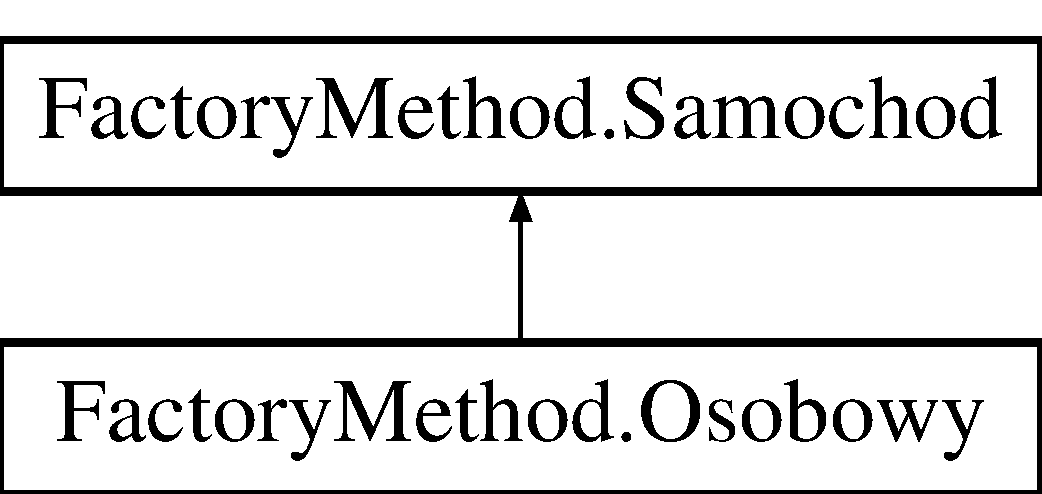
\includegraphics[height=2.000000cm]{class_factory_method_1_1_osobowy}
\end{center}
\end{figure}
\subsection*{Public Member Functions}
\begin{DoxyCompactItemize}
\item 
\mbox{\Hypertarget{class_factory_method_1_1_osobowy_a58a445d439d534e5ed01ec2369d0e3fc}\label{class_factory_method_1_1_osobowy_a58a445d439d534e5ed01ec2369d0e3fc}} 
void {\bfseries dodaj\+Osobowa\+Karoserie} ()
\item 
\mbox{\Hypertarget{class_factory_method_1_1_osobowy_ac2167fa6a5d1bed16bf0c4b5ab66e798}\label{class_factory_method_1_1_osobowy_ac2167fa6a5d1bed16bf0c4b5ab66e798}} 
void {\bfseries dodaj\+Klimatyzacje} ()
\item 
\mbox{\Hypertarget{class_factory_method_1_1_osobowy_ad47c1ea3189a40fb76dbb006aa9fc770}\label{class_factory_method_1_1_osobowy_ad47c1ea3189a40fb76dbb006aa9fc770}} 
override \hyperlink{class_factory_method_1_1_samochod}{Samochod} {\bfseries wyprodukuj\+Samochod} ()
\end{DoxyCompactItemize}
\subsection*{Additional Inherited Members}


\subsection{Detailed Description}
Produkt sprecyzowany 1 



The documentation for this class was generated from the following file\+:\begin{DoxyCompactItemize}
\item 
Program.\+cs\end{DoxyCompactItemize}

\hypertarget{class_factory_method_1_1_producent_samochodow}{}\section{Factory\+Method.\+Producent\+Samochodow Class Reference}
\label{class_factory_method_1_1_producent_samochodow}\index{Factory\+Method.\+Producent\+Samochodow@{Factory\+Method.\+Producent\+Samochodow}}


Producent tworzący obiekty na podstawie parametru about  


\subsection*{Public Member Functions}
\begin{DoxyCompactItemize}
\item 
\mbox{\Hypertarget{class_factory_method_1_1_producent_samochodow_a7339b0496f91acf51a421da86d5fadb7}\label{class_factory_method_1_1_producent_samochodow_a7339b0496f91acf51a421da86d5fadb7}} 
\hyperlink{class_factory_method_1_1_samochod}{Samochod} {\bfseries produkcja\+Samochodu} (String about)
\end{DoxyCompactItemize}


\subsection{Detailed Description}
Producent tworzący obiekty na podstawie parametru about 



The documentation for this class was generated from the following file\+:\begin{DoxyCompactItemize}
\item 
Program.\+cs\end{DoxyCompactItemize}

\hypertarget{class_factory_method_1_1_samochod}{}\section{Factory\+Method.\+Samochod Class Reference}
\label{class_factory_method_1_1_samochod}\index{Factory\+Method.\+Samochod@{Factory\+Method.\+Samochod}}


Ogolny produkt  


Inheritance diagram for Factory\+Method.\+Samochod\+:\begin{figure}[H]
\begin{center}
\leavevmode
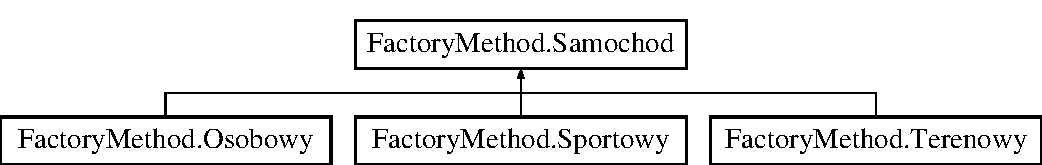
\includegraphics[height=2.000000cm]{class_factory_method_1_1_samochod}
\end{center}
\end{figure}
\subsection*{Public Member Functions}
\begin{DoxyCompactItemize}
\item 
\mbox{\Hypertarget{class_factory_method_1_1_samochod_a6e62670eb42c73db3e170ef3d017b20a}\label{class_factory_method_1_1_samochod_a6e62670eb42c73db3e170ef3d017b20a}} 
abstract \hyperlink{class_factory_method_1_1_samochod}{Samochod} {\bfseries wyprodukuj\+Samochod} ()
\end{DoxyCompactItemize}
\subsection*{Public Attributes}
\begin{DoxyCompactItemize}
\item 
\mbox{\Hypertarget{class_factory_method_1_1_samochod_a047ada1e3670069478edd62a77f53281}\label{class_factory_method_1_1_samochod_a047ada1e3670069478edd62a77f53281}} 
String {\bfseries about}
\end{DoxyCompactItemize}
\subsection*{Protected Member Functions}
\begin{DoxyCompactItemize}
\item 
\mbox{\Hypertarget{class_factory_method_1_1_samochod_a99d567a7c29de85f47acf79228ee9f32}\label{class_factory_method_1_1_samochod_a99d567a7c29de85f47acf79228ee9f32}} 
void {\bfseries dodaj\+Silnik\+I\+Skrzynie} ()
\end{DoxyCompactItemize}


\subsection{Detailed Description}
Ogolny produkt 



The documentation for this class was generated from the following file\+:\begin{DoxyCompactItemize}
\item 
Program.\+cs\end{DoxyCompactItemize}

\hypertarget{class_factory_method_1_1_sportowy}{}\section{Factory\+Method.\+Sportowy Class Reference}
\label{class_factory_method_1_1_sportowy}\index{Factory\+Method.\+Sportowy@{Factory\+Method.\+Sportowy}}


Produkt sprecyzowany 3  


Inheritance diagram for Factory\+Method.\+Sportowy\+:\begin{figure}[H]
\begin{center}
\leavevmode
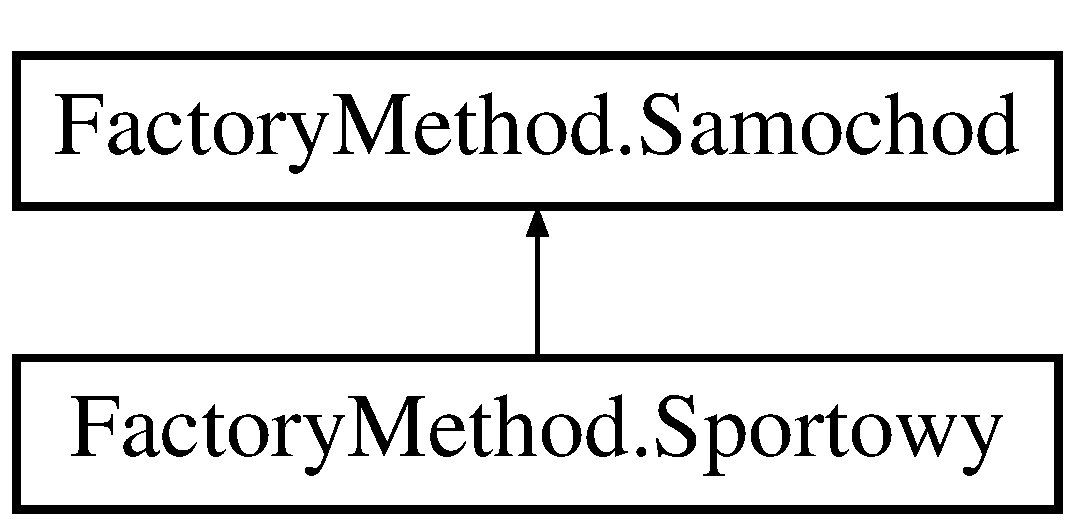
\includegraphics[height=2.000000cm]{class_factory_method_1_1_sportowy}
\end{center}
\end{figure}
\subsection*{Public Member Functions}
\begin{DoxyCompactItemize}
\item 
\mbox{\Hypertarget{class_factory_method_1_1_sportowy_aa96d8e877667cdd97e7d7803d568a581}\label{class_factory_method_1_1_sportowy_aa96d8e877667cdd97e7d7803d568a581}} 
void {\bfseries dodaj\+Sportowa\+Karoserie} ()
\item 
\mbox{\Hypertarget{class_factory_method_1_1_sportowy_a03980efb1c2a0975d22391b8e862717e}\label{class_factory_method_1_1_sportowy_a03980efb1c2a0975d22391b8e862717e}} 
void {\bfseries dodaj\+Turbo} ()
\item 
\mbox{\Hypertarget{class_factory_method_1_1_sportowy_afcee64a80c2622e4fc06360d8b4bd1d8}\label{class_factory_method_1_1_sportowy_afcee64a80c2622e4fc06360d8b4bd1d8}} 
override \hyperlink{class_factory_method_1_1_samochod}{Samochod} {\bfseries wyprodukuj\+Samochod} ()
\end{DoxyCompactItemize}
\subsection*{Additional Inherited Members}


\subsection{Detailed Description}
Produkt sprecyzowany 3 



The documentation for this class was generated from the following file\+:\begin{DoxyCompactItemize}
\item 
Program.\+cs\end{DoxyCompactItemize}

\hypertarget{class_factory_method_1_1_terenowy}{}\section{Factory\+Method.\+Terenowy Class Reference}
\label{class_factory_method_1_1_terenowy}\index{Factory\+Method.\+Terenowy@{Factory\+Method.\+Terenowy}}


Produkt sprecyzowany 2  


Inheritance diagram for Factory\+Method.\+Terenowy\+:\begin{figure}[H]
\begin{center}
\leavevmode
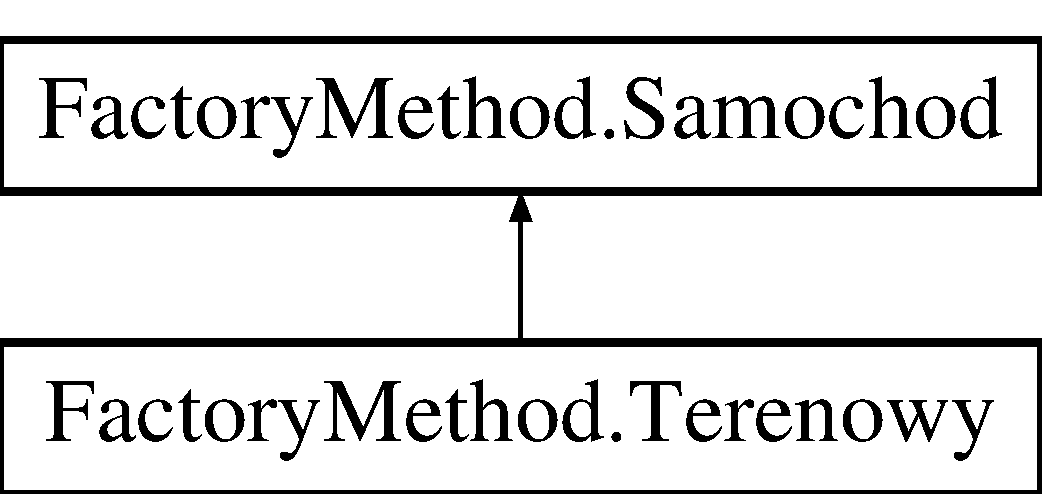
\includegraphics[height=2.000000cm]{class_factory_method_1_1_terenowy}
\end{center}
\end{figure}
\subsection*{Public Member Functions}
\begin{DoxyCompactItemize}
\item 
\mbox{\Hypertarget{class_factory_method_1_1_terenowy_ad80ba1863ae92a25a1dadd0786b82559}\label{class_factory_method_1_1_terenowy_ad80ba1863ae92a25a1dadd0786b82559}} 
void {\bfseries dodaj\+Terenowa\+Karoserie} ()
\item 
\mbox{\Hypertarget{class_factory_method_1_1_terenowy_ab619040153b6cdee28be46600372e68b}\label{class_factory_method_1_1_terenowy_ab619040153b6cdee28be46600372e68b}} 
void {\bfseries dodaj\+Terenowe\+Kola\+I\+Zawieszenie} ()
\item 
\mbox{\Hypertarget{class_factory_method_1_1_terenowy_af5a53d1c35602a406a3fcf25377b9ca2}\label{class_factory_method_1_1_terenowy_af5a53d1c35602a406a3fcf25377b9ca2}} 
void {\bfseries dodaj\+Klatke\+Bezpieczenstwa} ()
\item 
\mbox{\Hypertarget{class_factory_method_1_1_terenowy_a1ad06aaedf23b482a2258fba6da31315}\label{class_factory_method_1_1_terenowy_a1ad06aaedf23b482a2258fba6da31315}} 
override \hyperlink{class_factory_method_1_1_samochod}{Samochod} {\bfseries wyprodukuj\+Samochod} ()
\end{DoxyCompactItemize}
\subsection*{Additional Inherited Members}


\subsection{Detailed Description}
Produkt sprecyzowany 2 



The documentation for this class was generated from the following file\+:\begin{DoxyCompactItemize}
\item 
Program.\+cs\end{DoxyCompactItemize}

%--- End generated contents ---

% Index
\backmatter
\newpage
\phantomsection
\clearemptydoublepage
\addcontentsline{toc}{chapter}{Index}
\printindex

\end{document}
